\chapter{Baseline - Label Propagation}\label{chap:base}
\section{Label Propagation}
\label{sec:label_prop}
\par
Label propagation is a semi-supervised machine learning algorithm during which a node's label is propagated to its neighbours according to their proximity. The labelled data serve as sources to iteratively propagate labels through unlabelled data, allowing data that are not direct neighbours of labelled points to be labelled based on their unlabelled neighbours.\\

\subsection{Data Pre-processing}
\par
The input data are expected by the label propagation algorithm in a specific format and therefore our data have to be processed as follows before the actual algorithm starts.\\

\par
Let $(\mathcal{X}_1, l_1), \cdots, (\mathcal{X}_\ell, \cdots, l_\ell)$ be the labelled data and $(\mathcal{X}_{\ell+1}, l_{\ell+1}),\cdots,(\mathcal{X}_{\ell+u}, l_{\ell+u})$ the unlabelled data, i.e. $Y_U = \{l_{\ell+1}, \cdots l_{\ell+u} \}$ are unobserved. To estimate the labels of $Y_U$ from $\mathcal{X} = \{ \mathcal{X}_1,\cdots, \mathcal{X}_\ell, \mathcal{X}_{\ell+1},\cdots, \mathcal{X}_{\ell+u} \}$ and $Y_L = \{ l_1,\cdots, l_{\ell} \}$, we create a fully connected graph with nodes representing individual passenger's multivariate time series. We represent this graph by the adjacency matrix $W$, where the weight of the edge between nodes $i$ and $j$ is calculated as the similarity of time series $\mathcal{X}_i$ and $\mathcal{X}_j$, as described in \ref{similarity_computation}. Hence

\begin{align*}
    W_{ij} = sim(\mathcal{X}_i, \mathcal{X}_j)
\end{align*}

\par
Finally, we define a $(\ell+u)\times L$ label matrix $Y_0$, where $L$ represents the number of labels in our data set. $Y_{0_{il}}$ represents the probability of $i$-th data point holding the $l$-th label.\\


\subsection{The Algorithm}
\par
Once the input matrices has been prepared, the algorithm executes the following steps:
\begin{enumerate}
    \item Convert the adjacency matrix $W$ into a probabilistic transition matrix $T$, where $T_{ij}$ represents the probability of $i$ adopting the label of $j$:
    \begin{align*}
        T_{ij} = P(j \xrightarrow{} i) = \frac{W_{ij}}{\sum_{k=1}^{\ell+u}W_{kj}}
    \end{align*}
    
    \item Update the label probabilities by propagating 
    \begin{align*}
        Y_{t+1} = T\times Y_t;\quad t = \{0,1,2\cdots,n\}
    \end{align*}
    \item Row-normalise $Y_{t+1}$ to maintain the probability distribution representation:
    \begin{align*}
        Y_{{(t+1)}_{il}} = \frac{Y_{{(t+1)}_{il}}}{\sum_{k=1}^{L}Y_{{(t+1)}_{ik}}}
    \end{align*}
    \item Clamp observed data. Repeat from step 2 until $Y$ converges.
\end{enumerate}

During step 1, nodes propagate their labels based on the probabilities, resulting in the updated label matrix $Y_{t+1}$. During step 2, the rows of $Y_{t+1}$ are normalised to represent a probability distribution. In step 3, the labelled data points in $Y_{t+1}$ are set to their initial values to maintain their persistence and help unlabelled data during learning.

\par
After the iterative procedure terminates, the label matrix $Y_n$ is obtained from where the label with highest probability is used as the estimated label. Note that although the termination time $n$ is unknown, it is guaranteed that it converges in a finite number of iterations.\\

\begin{example}
    As an example, consider the following multivariate time series $\mathcal{X}_i$ with data \newline $\langle (t_1, c_1), \cdots, (t_n, c_n)\rangle$ on sensors $(X_{i,1}, \cdots, X_{i,m})$ and with labels $l_i$:
    
    \begin{figure}[H]
        \centering
        \begin{tabular}{|c|c|c|c|}
            \hline
             Time series & Sensor & Data & Label \\ \hline
             \multirow{3}{*}{$\mathcal{X}_1$} & $X_{1,1}$ & $\langle (0, 10), (1, 15), (2, 10)\rangle$ & \multirow{3}{*}{0} \\
                                              & $X_{1,2}$ & $\langle (0, 20), (1, 25), (2, 15)\rangle$ & \\
                                              & $X_{1,3}$ & $\langle (0, 20), (1, 15), (2, 20)\rangle$ & \\ \hline
             \multirow{3}{*}{$\mathcal{X}_2$} & $X_{2,1}$ & $\langle (0, 5), (1, 20), (2, 15)\rangle$ & \multirow{3}{*}{0} \\
                                              & $X_{2,2}$ & $\langle (0, 10), (1, 25), (2, 5)\rangle$ & \\
                                              & $X_{2,3}$ & $\langle (0, 15), (1, 5), (2, 10)\rangle$ & \\ \hline
             \multirow{3}{*}{$\mathcal{X}_3$} & $X_{3,1}$ & $\langle (0, 25), (1, 30), (2, 30)\rangle$ & \multirow{3}{*}{1} \\
                                              & $X_{3,2}$ & $\langle (0, 20), (1, 20), (2, 20)\rangle$ & \\
                                              & $X_{3,3}$ & $\langle (0, 10), (1, 5), (2, 10)\rangle$ & \\ \hline
             \multirow{3}{*}{$\mathcal{X}_4$} & $X_{4,1}$ & $\langle (0, 20), (1, 25), (2, 40)\rangle$ & \multirow{3}{*}{1} \\
                                              & $X_{4,2}$ & $\langle (0, 25), (1, 10), (2, 10)\rangle$ & \\
                                              & $X_{4,3}$ & $\langle (0, 15), (1, 45), (2, 25)\rangle$ & \\ \hline
             \multirow{3}{*}{$\mathcal{X}_5$} & $X_{5,1}$ & $\langle (0, 5), (1, 5), (2, 10)\rangle$ & \multirow{3}{*}{?} \\
                                              & $X_{5,2}$ & $\langle (0, 10), (1, 15), (2, 5)\rangle$ & \\
                                              & $X_{5,3}$ & $\langle (0, 25), (1, 20), (2, 35)\rangle$ & \\ \hline
        \end{tabular}
    \end{figure}
    
    Firstly, we construct the similarity matrix $W$ which represents the fully connected graph of passengers.
    
    Given that weight between nodes $i$ and $j$ is calculated as $w_{ij} = sim(X_i, X_j)$, we obtain:
    \begin{align*}
        W = 
        \begin{bmatrix}
            1    & 0.95 & 0.25 & 0.15 & 0.80 \\
            0.95 & 1    & 0.30 & 0.25 & 0.85 \\
            0.25 & 0.30 & 1    & 0.95 & 0.20 \\
            0.15 & 0.25 & 0.95 & 1    & 0.10 \\
            0.80 & 0.85 & 0.20 & 0.10 & 1
        \end{bmatrix}
    \end{align*}
    
    To transform $W$ into probabilistic transition matrix $T$, we row-normalise the matrix:
    \begin{align*}
        T_{ij} = \frac{W_{ij}}{\sum_{k=1}^{5}W_{kj}}
    \end{align*}
    
    Therefore, the probabilistic transition matrix $T$ looks as follows.
    \begin{align*}
        T = 
        \begin{bmatrix}
            0.317 & 0.283 & 0.094 & 0.061 & 0.271 \\
            0.302 & 0.299 & 0.111 & 0.102 & 0.288 \\
            0.079 & 0.089 & 0.370 & 0.388 & 0.068 \\
            0.048 & 0.075 & 0.352 & 0.408 & 0.034 \\
            0.254 & 0.254 & 0.074 & 0.041 & 0.339
        \end{bmatrix}
    \end{align*}
    
    Construction of label matrix $Y$ is straightforward. Note that unobserved data can be initialised with any probability.
    
    \begin{align*}
        Y_0 = 
        \begin{bmatrix}
            1   & 0 \\
            1   & 0 \\
            0   & 1 \\
            0   & 1 \\
            0.5 & 0.5 
        \end{bmatrix}
    \end{align*}
    
    Finally, the iterative algorithm can start. In the first step, we propagate $Y \xleftarrow{} TY$:
    
    \begin{align*}
        Y_1 =
        \begin{bmatrix}
            0.317 & 0.283 & 0.094 & 0.061 & 0.271 \\
            0.302 & 0.299 & 0.111 & 0.102 & 0.288 \\
            0.079 & 0.089 & 0.370 & 0.388 & 0.068 \\
            0.048 & 0.075 & 0.352 & 0.408 & 0.034 \\
            0.254 & 0.254 & 0.074 & 0.041 & 0.339
        \end{bmatrix}
        \times
        \begin{bmatrix}
            1   & 0 \\
            1   & 0 \\
            0   & 1 \\
            0   & 1 \\
            0.5 & 0.5 
        \end{bmatrix}
        = 
        \begin{bmatrix}
            0.7355 & 0.2905 \\
            0.7450 & 0.3570 \\
            0.2020 & 0.7920 \\
            0.1400 & 0.7770 \\
            0.6775 & 0.2845
        \end{bmatrix}
    \end{align*}
    
    In step two, we have to row-normalise the newly obtained $Y$:
    \begin{align*}
        Y_1 =
        \begin{bmatrix}
            0.7168 & 0.2832 \\
            0.6760 & 0.3240 \\
            0.2032 & 0.7968 \\
            0.1527 & 0.8473 \\
            0.7042 & 0.2958
        \end{bmatrix}
    \end{align*}
    
    And finally, we clamp the labelled data to their original values, obtaining
    \begin{align*}
        Y_1 =
        \begin{bmatrix}
            1      & 0      \\
            1      & 0      \\
            0      & 1      \\
            0      & 1      \\
            0.7042 & 0.2958
        \end{bmatrix}
    \end{align*}
    
    This procedure is repeated until the values of $Y_n$ converge, giving us the result
    \begin{align*}
        Y_n =
        \begin{bmatrix}
            1      & 0      \\
            1      & 0      \\
            0      & 1      \\
            0      & 1      \\
            0.8154 & 0.1846
        \end{bmatrix}
    \end{align*}
    
    Therefore, the time series $\mathcal{X}_5$ is predicted to carry label $1$ with probability $0.8154$ and label $0$ with probability $0.1846$.
\end{example}

\section{Similarity computation}
\label{similarity_computation}
\par
In order to be able to transform our data to the input graph form required for label propagation, we first need to introduce a similarity function.
\par
\medskip
Given the multidimensional time-series for two mobile devices, $\mathcal{X}_a$ and $\mathcal{X}_b$, we can build the tables $T_a$ and $T_b$, using the procedure defined in \cref{chap:datamodelling}, with each table being initialised with the shape $m \times n$, where $m$ is the number of sensors and $n$ is the overall latest time stamp from $\mathcal{X}_a$ or $\mathcal{X}_b$. The similarity function $sim$ should then compare $T_a$ and $T_b$, resulting in a similarity measure $sim(T_a,T_b)$ in the interval [0,1].
\par
\medskip
\par
First, we need to calculate the overall distance between $T_a$ and $T_b$. The data for each mobile device consists of a set of time-series, each corresponding to the data for one sensor, represented as a column in the table. Based on that we can calculate a distance for every sensor (column) in the table as the sum of cell-by-cell differences. These sensor distances can be summed further, resulting in a single distance value between $T_a$ and $T_b$.\\

\par
Overall, we can define this calculation for tables $T_a$ and $T_b$, both of shape $n \times m$ as the following absolute-valued matrix difference of table values:
\begin{equation*}
    dist(T_a,T_b) = \sum_{i=1}^n \sum_{j=1}^m |{T_a}_{i,j} - {T_b}_{i,j}|
\end{equation*}
where
\begin{itemize}
    \item $n$ is the number of rows in tables $T_a$, $T_b$
    \item $m$ is the number of columns in tables $T_a$, $T_b$
    \item ${T_a}_{i,j}$ is the value in the $i$-th row and $j$-th column of $T_a$
    \item ${T_b}_{i,j}$ is the value in the $i$-th row and $j$-th column of $T_b$
\end{itemize}

\par
Now, in order to transform the absolute distance into a similarity measure in the interval [0,1], we can normalise the distance using the maximum possible distance between two tables:
\begin{equation*}
    sim(T_a,T_b) = \frac{dist_{max} - dist(T_a,T_b)}{dist_{max}}
\end{equation*}
where $dist_{max}$ can be calculated as:
\begin{equation*}
    dist_{max} = n \cdot m \cdot v_{max}
\end{equation*}
where $v_{max}$ is the maximum absolute value of a cell in a table of shape $n \times m$.\\

\par
To illustrate this, we can use the table in \cref{fig:datamodelling:tables:3} on page \pageref{fig:datamodelling:tables:3}. We know that the absolute value of a cell will never be higher than 75, therefore we let $v_{max}$ be 75. As the table contains 3 columns (sensors) and 10 rows (time), we calculate $dist_{max}$ as $n \cdot m \cdot v_{max} = 10 \cdot 3 \cdot 75 = 2250$. 

\par
The intuition behind using $dist_{max}$ is to define the global hypothetical maximum for any similarity computation in our data, given the shape of the pre-processed mobile address table models. The $dist_{max}$ then serves as a common constant, with distances being normalised into a similarity interval of [0,1], relative to this constant.

\par
An overview of the similarities calculated using $sim(T_a,T_b)$ on our data may be seen in \cref{fig:results:similarity_distribution} of the results section of the report.


\section{Results}
In order to test label propagation on our data, we have applied the similarity computation formulated in the previous section to calculate the similarities for a portion of our data set.\par
\medskip
We have selected 275 mobile addresses per class, representing the total of 1100 nodes in the input graph for label propagation. The similarity computation was then performed on each of the 604450 edges in the graph (each pair of mobile addresses) to obtain the adjacency matrix $W_{ij}$. The distribution of similarity scores between all the compared pairs of addresses may be seen in Figure \ref{fig:results:similarity_distribution}. \par

\begin{figure}[H]
    \centering
    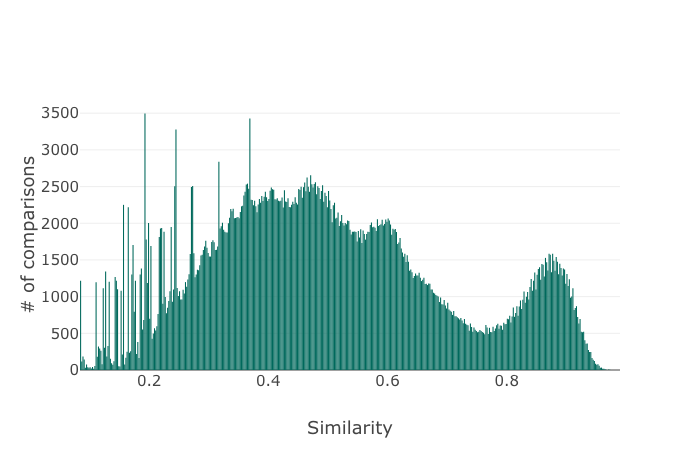
\includegraphics[width=.7\textwidth]{Pictures/similarity_distribution_plot.png}
    \caption{Distribution of similarity scores calculated from all pairs of 1100 addresses, using the similarity computation $sim(T_a,T_b)$ from Section \ref{similarity_computation}}
    \label{fig:results:similarity_distribution}
\end{figure}

\medskip
For training data (seeds), we have selected 90 addresses for each class (360 addresses in total, corresponding to roughly 1/3 of unique addresses in the input graph), for which we have defined ground truth labels $Y_L$.\par
\medskip

Given this configuration, running the model on the test data resulted in an overall accuracy of 36\%, and per-label accuracies of 37\%, 3\%, 67\% and 40\% for "manual", "staff", "no-q" and "privium" respectively. A more detailed breakdown of how the model predicted different examples in test data may be seen in the confusion matrix below.

\begin{figure}[H]
    \centering
    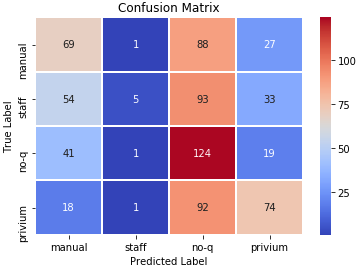
\includegraphics[width=.5\textwidth]{Pictures/label_prop_confusion.png}
    \caption{Label propagation results (confusion matrix)}
    \label{fig:label_prop:confusion_matrix}
\end{figure}
\pagebreak

\subsection{Performance metrics}
\label{section:performance_metrics}
\subsubsection{Confusion matrix}
The confusion matrix from Figure \ref{fig:label_prop:confusion_matrix} gives a representation of the relationship between the ground truth and the predicted labels for each example in the test data. The rows in the matrix represent the true labels, while the columns represent the predicted labels. Inherently, the diagonal of the matrix represents the numbers of correctly classified examples for each label. Similarly, the tile in the fourth row and first column of the confusion matrix gives the number of examples where the true label was "privium", but the classifier predicted "manual".

\subsubsection{True positive, False positive, False negative and True negative}
\label{sec:true_positives}
For each label, we can also define the following measures, based on the confusion matrix:
\begin{itemize}
    \item \textbf{True positives (TP)} are the examples for which the true label was also the predicted label. Considering the confusion matrix $CM$:
        \begin{equation*}
            TP_l = CM_{l,l}
        \end{equation*}
    where $CM_{ll}$ is the value in the $l$-th row and $l$-th column of $CM$.
    
    \item \textbf{False positives (FP)} for label $l$ are all the examples that are not $l$, but were classified as $l$. Given the confusion matrix $CM$:
        \begin{equation*}
            FP_l = \sum_k CM_{k,l} - CM_{l,l}
        \end{equation*}
    where $CM_{k,l}$ is the value in the $k$-th row, $l$-th column of $CM$ and $CM_{l,l}$ is the value in the $l$-th row, $l$-th column of $CM$.
    
    \item \textbf{False negatives (FN)} for label $l$ are the examples with true label $l$ that have not been classified as $l$. In terms of confusion matrix $CM$:
    \begin{equation*}
        FN_l = \sum_k CM_{l,k} - CM_{l,l}
    \end{equation*}
    where $CM_{l,k}$ is the value in the $l$-th row, $k$-th column of $CM$ and $CM_{l,l}$ is the value in the $l$-th row, $l$-th column of $CM$.
    
    \item \textbf{True negatives (TN)} with respect to label $l$ are those examples for which the true label is not $l$, nor have they been classified as $l$. Given confusion matrix $CM$:
    \begin{equation*}
        TN_l = \sum_j\sum_k CM_{j,k} \quad j,k \neq l
    \end{equation*}
\end{itemize}

An illustration of these concepts ($TP$, $FP$, $FN$ and $TN$) on a confusion matrix for a given label (\textit{manual}) may be seen in \cref{fig:manual_tp_fn_tn_etc_example} below. 

\begin{figure}[H]
    \centering
    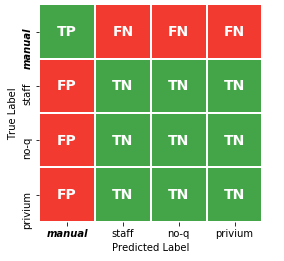
\includegraphics[width=.4\textwidth]{Pictures/manual_tp_fn_tn_example.png}
    \caption{$TP$, $FP$, $FN$ and $TN$ values illustrated on the confusion matrix for label \textit{manual}}
    \label{fig:manual_tp_fn_tn_etc_example}
\end{figure}

\subsubsection{Accuracy, recall and precision}
Given our true and predicted test data examples, we can calculate the (overall) \textbf{accuracy} simply as:
\begin{equation*}
    Accuracy = \frac{\text{Correctly Predicted Examples}}{\text{Total Examples}}
\end{equation*}
which can be calculated using the confusion matrix $CM$ as:
\begin{equation*}
    Accuracy = \frac{\sum\limits_{i=1}^{4} CM_{i,i}}{\sum\limits_{i=1}^{4}\sum\limits_{j=1}^{4} CM_{i,j}}
\end{equation*}
where $CM_{i,i}$ and $CM_{i,j}$ are the values of matrix $CM$ in the $i$-th row, $i$-th column and $i$-th row, $j$-th column respectively.\par
\medskip
\par
We will also define two concepts for measuring performance per-label: \textit{recall} and \textit{precision}.
\medskip
\par
\textbf{Recall} is the ratio of correctly predicted examples relative to all true examples of a given label in the test data, or mathematically, given the confusion matrix $CM$:  
\begin{equation*}
    Recall(l) = \frac{CM_{l,l}}{\sum\limits_{k=1}^{4} CM_{l,k}} = \frac{TP_l}{TP_l+FN_l}
\end{equation*}
where $l$ is number of a label with respect to rows and columns in the confusion matrix, $TP_l$ is the number of true positives and $FN_l$ the number of false negatives (\cref{sec:true_positives}).

\medskip
\par
\textbf{Precision} is the ratio of correctly predicted examples relative to the total of examples predicted for that label (correct and incorrect), or mathematically, given the confusion matrix $CM$:

\begin{equation*}
    Precision(l) = \frac{CM_{l,l}}{\sum\limits_{k=1}^{4} CM_{k,l}} = \frac{TP_l}{TP_l + FP_l}
\end{equation*}
where $l$ is number representation of a label with respect to rows and columns in the confusion matrix, $TP_l$ is the number of true positives and $FP_l$ is the number of false positives (\cref{sec:true_positives}). 

\subsection{Performance summary}
Having defined the performance measures, below is the performance summary for label propagation on our data, derived from the confusion matrix in Figure \ref{fig:label_prop:confusion_matrix}. 
\begin{table}[H]
    \centering 
    \begin{tabular}{c|c|c|c|}
        \cline{2-4}
                                                     & \textbf{Precision} & \textbf{Recall} & \textbf{Examples} \\ \hline
        \multicolumn{1}{|l|}{\textbf{manual}}        & 0.38               & 0.37            & 185               \\ \hline
        \multicolumn{1}{|l|}{\textbf{staff}}         & 0.62               & 0.03            & 185               \\ \hline
        \multicolumn{1}{|l|}{\textbf{no-q}}          & 0.31               & 0.67            & 185               \\ \hline
        \multicolumn{1}{|l|}{\textbf{privium}}       & 0.48               & 0.40            & 185               \\ 
        \hline \hline
        \multicolumn{1}{|l|}{\textbf{Average / Total}} & 0.45               & 0.37            & 740               \\ 
        \hline \hline
        \multicolumn{1}{|l|}{\textbf{Accuracy}}      & \multicolumn{3}{c|}{0.36}                                \\ \hline
    \end{tabular}   
    \caption{Performance summary for label propagation}
\end{table}
\subsection{Interpretation and Conclusion}
As the previous section regarding results presents, the accuracy of our label propagation model is low and unsatisfactory. While testing the model we have experimented with different variations of computing the similarity, which yielded similar results. \par
\medskip
We attribute this to the nature of our data set. The readings recorded by sensors for a single mobile device tend to contain few data points, scattered at different times. This makes most of the simple, generic time-series distance measures inaccurate, which in consequence negatively affects the performance of label propagation. Better similarity computations could be devised, but would likely require more advanced time-series analysis and possibly feature engineering. \par
\medskip
It is for this reason that we have decided to move away from label propagation and other models requiring distance measures and we will explore different approaches going forward.


